\documentclass[11pt,letterpaper]{article}
\usepackage{fullpage}
\usepackage[top=2cm, bottom=4.5cm, left=2.5cm, right=2.5cm]{geometry}
\usepackage{amsmath,amsfonts,amssymb}
\usepackage{lastpage}
\usepackage[inline]{enumitem}
\usepackage{fancyhdr}
\usepackage{mathrsfs}
\usepackage{xcolor}
\usepackage{graphicx}
\usepackage{subcaption}
\usepackage{appendix}
\usepackage{hyperref}
\usepackage{titlesec}
\usepackage{fancyvrb}
\hypersetup{ colorlinks=true, linkcolor=blue, linkbordercolor={0 0 1}}

\renewcommand{\arraystretch}{1.5}
\titlespacing*{\section}{0pt}{0.65\baselineskip}{0.5\baselineskip}

\setlength{\parindent}{0.0in}
\setlength{\parskip}{0.05in}

\newcommand{\qrf}{\texttt{QRFactor} }

\pagestyle{fancyplain}
\lhead{}
\chead{GPU Solutions for PSCAD: IT17112}
\rhead{}
\cfoot{\small\thepage}
\headsep 32pt

%%%%%%%%%%%%%%%%%%%%%%%%%%%%%%%%%%%%%%%%%%%%%%%%%%%%%%%%%%%%%%%%%%%%%%%%%%%%%%%
%%%%%%%%%%%%%%%%%%%%%%%%%%%%%%%%%%%%%%%%%%%%%%%%%%%%%%%%%%%%%%%%%%%%%%%%%%%%%%%

\begin{document}
\begin{center}
    {\Large \bf Monthly Summary: May, 2020}
\end{center}

The summary covers progress made during both April and May of 2020. Following the latest
update of the \verb+QRFactor+ code to utilize sparse matrix solving, a full run of the \emph{Province}
data set was undertaken using a laptop with an NVIDIA Quadro RTX 3000 GPU. Timings were collected for
the one-time matrix factorization and solving of the factored system at each time step. 
In figure~\ref{f:timings}, we see that the average time to 
solve the system $R\mathbf{x}(t) = Q^T \mathbf{b}(t)$ for each time step is approximately $2.35$ ms.
As stated previously, this represents a speedup of roughly 4.5x at each time step. Furthermore, by using
the sparse matrix version of the QR factorization method, a speedup of roughly 35x is achieved.

\begin{figure}[ht]
    \centering
    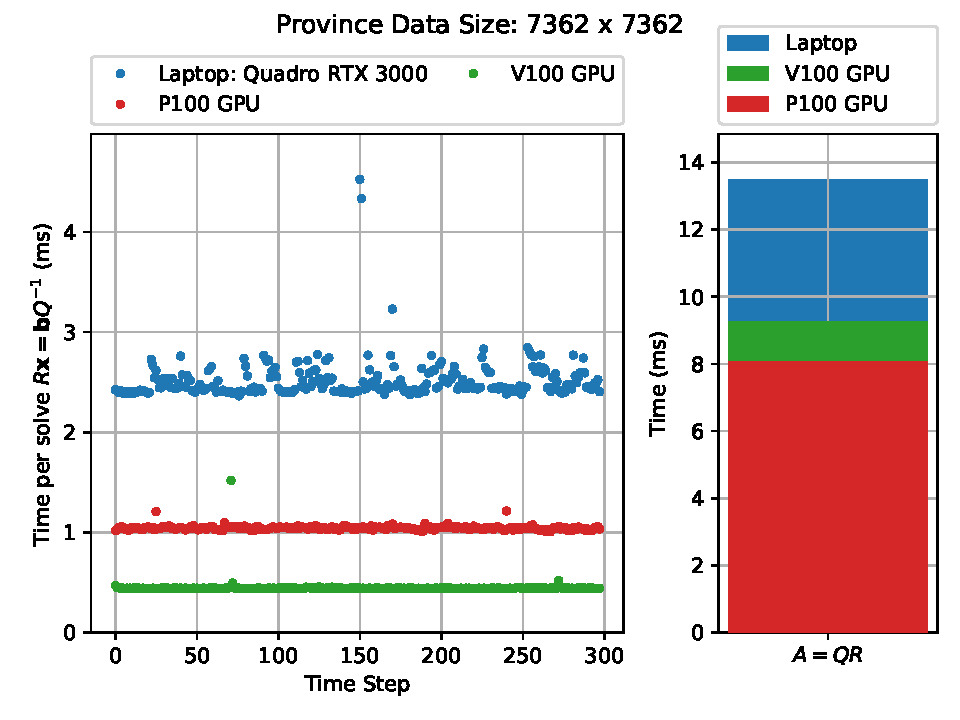
\includegraphics[width=0.75\textwidth]{C:/Users/bradc/Documents/MHI/Output/FullTimings}
    \caption{Timings for solving $\mathbf{x}(t)$ over the entire \emph{Province} data set 
    after the matrix $A$ has been factored}
    \label{f:timings}
\end{figure}

In anticipation of presenting a working test model to MHI, a set of instructions for building
\qrf on both Windows systems and Linux systems was written. For Windows systems, the code was built using
Microsoft Visual Studio 2019 while Linux systems relied on Docker containers. These instructions included 
screen shots of the relevant options and sample scripts for setting up the environments. Please see the 
document QRFactorInstructions.pdf for more details.

%%%%%%%%%%%%%%%%%%%%%%%%%%%%%%%%%%%%%%%%%%%%%%%%%%%%%%%%%%%%%%%%%%%%%%%%%%%%%%%

\section*{Moving to U of W Servers}

While the timings from running the code on a laptop were an improvement over previous results, the hardware
available on the U of W servers (NVIDIA's Tesla P100-PCIE-12GB GPU) will provide the most accurate measure of 
performance. In order to run \qrf on these servers, however, a transition to a Docker container environment was
needed. During April and May, familiarity with Docker and Docker containers became essential. With this 
new knowledge, a custom image was created based off of NVIDIA's own CUDA image. The CUDA Toolkit -- which 
does not come with the NVIDIA image -- was added, as were additional useful packages. From this custom
image, a container running Ubuntu 18.04 that was able to interface with the underlying GPUs could be created
and attached to at any time. An explanation of the benifits of working with containers, as well as an introduction 
to Docker itself, is available through their \href{https://docker.com}{website}. Now that the container
environment has been created, debugging is ongoing and new timings will be available soon.


%%%%%%%%%%%%%%%%%%%%%%%%%%%%%%%%%%%%%%%%%%%%%%%%%%%%%%%%%%%%%%%%%%%%%%%%%%%%%%%

\section*{Verification of Results}

While the GPU-based methods had already provided significant speedups, it was still important to verify that the 
code was functioning properly. To that end, we were provided with the output from the first 223 time steps produced
by MHI's version of the solver for the \emph{Province} data. We also compared random outputs of the GPU-based solution 
from \qrf to CPU-based solutions. We found that a typical relative difference between \qrf GPU and CPU results was on
the order of 10$^{-15}$, with a small number of values differing by up to 10$^{-9}$. One surprise, however, was the 
existence of three lines of output -- lines 2208 to 2210 -- that consistently gave relative differences on the order 
of 10$^{-3}$. After consulting with MHI, we were told that this was a known issue with the set up of the
test data, and not an indication of an issue with \qrf\!\!.

%%%%%%%%%%%%%%%%%%%%%%%%%%%%%%%%%%%%%%%%%%%%%%%%%%%%%%%%%%%%%%%%%%%%%%%%%%%%%%%
%%%%%%%%%%%%%%%%%%%%%%%%%%%%%%%%%%%%%%%%%%%%%%%%%%%%%%%%%%%%%%%%%%%%%%%%%%%%%%%































\end{document}
